\section{Auswertung}
\label{sec:Auswertung}

%\begin{figure}
%  \centering
%  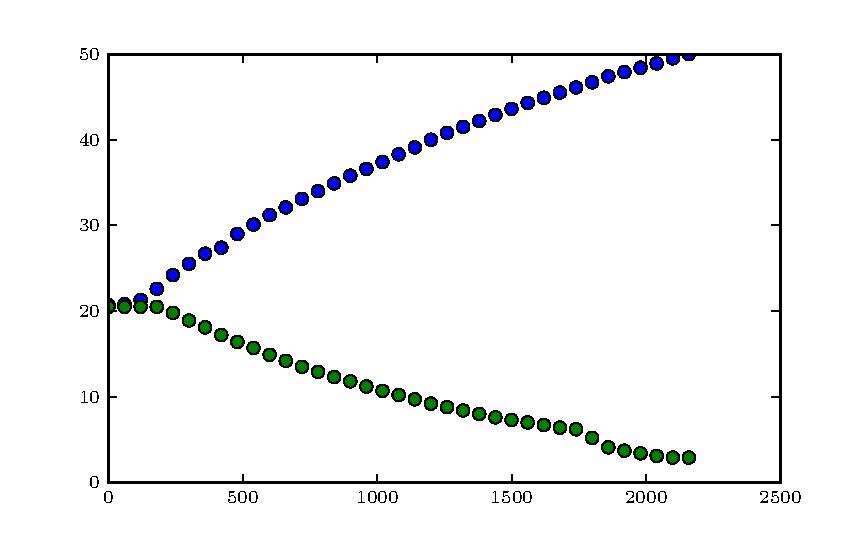
\includegraphics{plot.pdf}
%  \caption{Plot.}
%  \label{fig:plot}
%\end{figure}
\subsection{Konfiguration des Messprogramms}
\begin{figure}
  \centering
  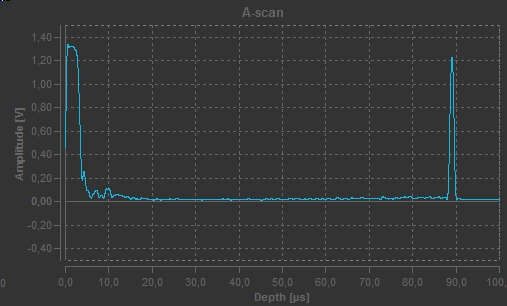
\includegraphics{Messdaten/a.jpg}
  \caption{Plot.}
  \label{fig:a1}
\end{figure}
Zur Bestimmung der Schallgeschwindigkeit im Material der vorliegenden Acrylzylinder wird die Länge eines Zylinders vermessen und die Zeitdifferenz $\Delta t$ zwischen zwei Impulsen bestimmt.
In Abbildung \ref{fig:a1} ist der Amplituden-Scan der Messung dargestellt.
Die Zeitdifferenz zwischen den beiden Maxima wird mithilfe der Cursor bestimmt zu
\begin{equation}
  \Delta t=\SI{88.69}{\micro\second} \text{.}
\end{equation}
Die Amplitudenhöhe wurde nicht vermessen, da nicht bekannt ist, wie die Verstärkung des Signals herausgerechnet werden muss.
Über die gemessene Länge des Acrylzylinders $l=\SI{120.5}{\milli\meter}$ ergibt sich mit Formel \eqref{eqn:laufzeit} eine Schallgeschwindigkeit von
\begin{equation}
  v_{\mathrm{Schall}}=\SI{2717.33}{\meter\per\second} \text{.}
\end{equation}
Da es zahlreiche unterschiedliche Literaturwerte für die Schallgeschwindigkeit in Acryl gibt, wird, dem Messergebnis folgend, für die weiteren Messungen eine Schallgeschwindigkeit von $v_{\mathrm{Schall}}=\SI{2720}{\meter\per\second}$ in das Messprogramm eingetragen.
Mit diesem Wert ist das Programm schließlich in der Lage, die Eindringtiefe der Schallwelle in das Material zu bestimmen.
Der Abstand zwischen den beiden Peaks entspricht dann der Länge des Acrylstabs.
Die durch das Programm berechnete Länge ergibt sich zu
\begin{equation}
  l=\SI{119.726}{\milli\meter} \text{.}
\end{equation}
\FloatBarrier

\subsection{Schallgeschwindigkeit mit dem Durchschallungsverfahren}
\begin{figure}
  \centering
  \includegraphics{Messdaten/d.pdf}
  \caption{Plot.}
  \label{fig:durchschall}
\end{figure}
\FloatBarrier

\subsection{Schallgeschwindigkeit über Impuls-Echo-Verfahren}
\begin{figure}
  \centering
  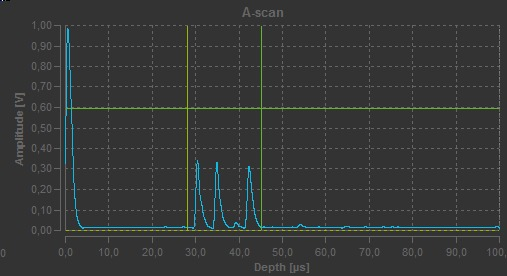
\includegraphics{Messdaten/ascan.pdf}
  \caption{Plot.}
  \label{fig:iev}
\end{figure}
\FloatBarrier
\subsection{Bestimmung der Dämpfung mit dem Impuls-Echo-Verfahren}
\begin{figure}
  \centering
  \includegraphics{Messdaten/amplitude.pdf}
  \caption{Plot.}
  \label{fig:daempf}
\end{figure}
\FloatBarrier

%%%%%%%%%%%%%%%
\subsection{Auge}

Abstand Hornhaut Anfang Linse:  $\SI{6,2604}{\milli\meter}$
Avstand Hornhaut Ende Linse=  $\SI{16,0979}{\milli\meter}$
Abstand Hornhaut Retina=  $\SI{21,329}{\milli\meter}$
